\documentclass[a4paper, 10pt, final, garamond]{book}
\usepackage{cours-preambule}
\graphicspath{{./figures/}}

\makeatletter
\renewcommand{\@chapapp}{Contr\^ole de connaissances}
\makeatother

% \toggletrue{student}
% \toggletrue{corrige}
\renewcommand{\mycol}{black}
% \renewcommand{\mycol}{gray}

\begin{document}
\setcounter{chapter}{19}

\settype{enon}
\settype{solu}

\chapter{Forces centrales et solides\ifstudent{~(12')}}

\begin{enumerate}[label=\sqenumi]
	\nitem{7}%
	Soit un point M soumis à une unique force centrale $\Ff$. Démontrer que son
	moment cinétique se conserve, justifier que son mouvement est plan et
	démontrer la loi des aires à l'aide d'un schéma. Pas besoin d'introduire la
	constante des aires.
	\smallbreak
	\begin{isd}
		\psw{
			Force centrale $\stm[-1]{\Lra} \Ff \parr \OM \Ra \Mcf_{\Or}(\Ff) = \OM \wedge \Ff =
				\of$
			\begin{gather*}
				\beforetext{TMC~:}
				\boxed{\dv{\Lcf_{\Or}}{t} \stm[-1]{=} \of}
				\Lra
				\Lcf(0) = \Lc_0 \uz \stm{=} \Lcf(t)
				\\
				\beforetext{Ainsi,}
				\boxed{\OM(t) \wedge m\vf(t) \stm[-1]{=} \Lc_0 \uz} \quad \forall t
			\end{gather*}
			\smallbreak
			Pendant une durée $\dd{t}$, le point M balaye une aire $\dd{\Ac}$
			\begin{gather*}
				\dd{\Ac}            \stm{=} \frac{1}{2}\norm{\OM \wedge \vf \dd{t}}
				\Lra
				\dd{\Ac}            = \frac{1}{2}\norm{\OM \wedge m \vf} \frac{\dd{t}}{m}
				\\\Lra
				\boxed{\dv{\Ac}{t} \stm{=} \frac{\norm{\Lcf_{\Or}}}{2m} = \cte}
				\qed
			\end{gather*}
		}
		\vspace{-15pt}
		\tcblower
		\begin{center}
			\sswitch{
				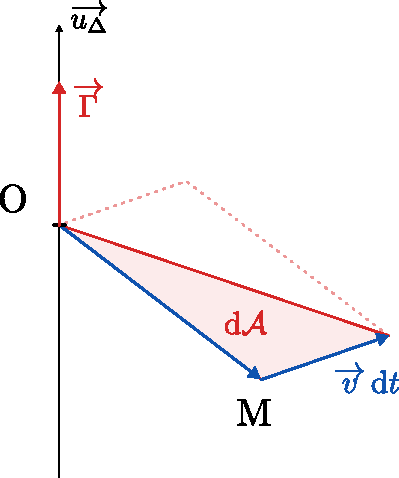
\includegraphics[scale=.6, draft=true]{dAmomcin}
			}{
				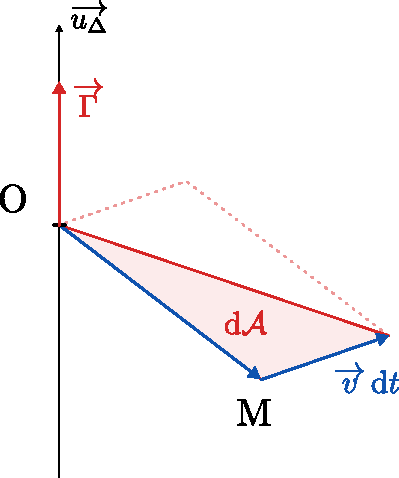
\includegraphics[scale=.6]{dAmomcin}
			}
			\captionof{figure}{Moment cinétique et aire balayée\protect\pt{1}}
		\end{center}
	\end{isd}
	\nitem{4}%
	Compléter le tableau de comparaison suivant~:
	\begin{table}[htbp!]
		\centering
		\caption{Analogie mécanique du point et solide \xul{en rotation}}
		\begin{tabularx}{\linewidth}{|l|c|c|Y|c|Y|c|c|}
			\hline
			                                                  &
			Inertie                                           &
			Déplac\mnt                                        &
			Quantité                                          &
			Causes                                            &
			Évolu$^\circ$                                     &
			$\Ec_c$                                           &
			$\Pc$
			\\\hline
			\rotatebox[origin=c]{90}{Point}                   &
			\psw{$m$}                                         &
			\psw{$\vf$}                                       &
			\psw{$\pf = m\vf$}                                &
			\psw{$\Ff$}                                       &
			\psw{$\DS \dv{\pf}{t} = \Ff_{\ext}$}              &
			\psw{$\frac{1}{2}mv^2$}                           &
			\psw{$\Ff \cdot \vf$}\tikzmark{PP}
			\\[1em]\hline
			\rotatebox[origin=c]{90}{Solide}                  &
			\psw{$J_{\D}$}                                    &
			\psw{$\wf$}                                       &
			\psw{$\Lcf = \OM \wedge \pf = J_{\D}\wf$}         &
			\psw{$\Mcf = \OM \wedge \Ff$}                     &
			\psw{$\DS \dv{\Lcf_{\Or}}{t} = \Mcf_{\Or, \ext}$} &
			\psw{$\frac{1}{2}J_{\D}\w^2$}                     &
			\psw{$\Mcf \cdot \wf$}\tikzmark{PS}
			\\[1em]\hline
		\end{tabularx}
	\end{table}
	\tikz[remember picture, overlay]
	\node[right=20pt of pic cs:PP] {\pt{2}}
	;
	\tikz[remember picture, overlay]
	\node[right=18pt of pic cs:PS] {\pt{2}}
	;
	\nitem{10}%
	Compléter le schéma du pendule pesant avec les forces et leurs moments,
	calculés \textbf{par le bras de levier}. On suppose la liaison pivot parfaite.
	Trouver alors l'équation du mouvement par application du \textbf{TMC scalaire
		d'abord} puis \textbf{TPC ensuite}.
	\smallbreak
	\vspace{-15pt}
	\noindent
	\begin{minipage}[t]{0.70\linewidth}
		\psw{
			\begin{enumerate}[label=\sqenumi]
				\bitem{\tikzmark{SP}Système}~: \{pendule\} solide indéformable de masse $m$
				\bitem{Référentiel}~: terrestre, supposé galiléen.
				\bitem{\tikzmark{RP}Repère}~:
				cylindrique $(\Or,\er,\et,\ez)$ avec O centre de la liaison pivot.
				\bitem{Repérage}~: $\OG = d\er$
				\bitem{Bilan des actions}~:
				\vspace{-15pt}
				\[
					\begin{array}{lcc}
						\qquad\textbf{Origine}  & \textbf{Force}          & \textbf{Moment}
						\\
						\textbf{Poids}          & \quad \Pf = m\gf \quad~ & \Mc_z(\Pf) \stm[-1]{=}
						-mgd \sin(\th)
						\\
						\textbf{Pivot parfaite} & \of                     & \vv{\G} \stm[-1]{=} \of
					\end{array}
				\]
			\end{enumerate}
		}
		\vspace{-15pt}
	\end{minipage}
	\hfill
	\begin{minipage}[t]{0.25\linewidth}
		\vspace{0pt}
		\begin{center}
			\sswitch{
				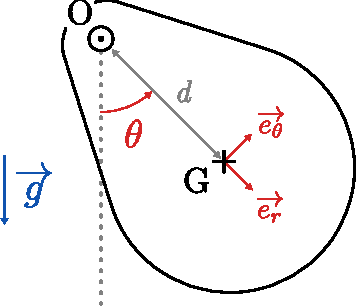
\includegraphics[width=\linewidth]{ppesant}
			}{
				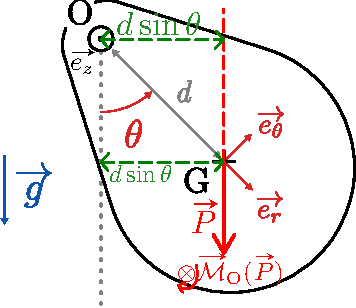
\includegraphics[width=\linewidth]{ppesant_complet}
			}
			\vspace{-15pt}
			\captionsetup{justification=centering}
			\captionof{figure}{\\Pendule pesant\protect\pt{1}}
		\end{center}
	\end{minipage}
	\tikz[remember picture, overlay]
	\node[below left=0pt and 20pt of pic cs:SP] {\pt{1}}
	;
	\tikz[remember picture, overlay]
	\node[below left=0pt and 20pt of pic cs:RP] {\pt{1}}
	;
	\psw{
		\begin{enumerate}[label=\sqenumi, start=6]
			\bitem{TMC}~:
			\vspace{-20pt}
			\[
				\dv{\Lc_z}{t} \stm{=} J_z \tpp = \Mc_z(\Pf)
				\Lra
				\boxed{\tpp + \frac{mgd}{J_z} \sin(\th) \stm{=} 0}
			\]
			\vspace{-15pt}
			\bitem{TPC}~: on calcule $\Ec_c$ et $\Pc$~:
			\begin{gather*}
				\Ec_c = \frac{1}{2}J_z \w^2
				\stm{\qet}
				\Pc(\Pf) = \Mc_z(\Pf)\w
				\quad \Ra \quad
				\dv{\Ec_c}{t} \stm{=} \Pc(\Pf)
				\Lra
				J_z \dot{\w} \cancel{\w} \stm{=} -mgd\sin(\th)\cancel{\w}
				\Lra
				\boxed{\tpp + \frac{mgd}{J_z}\sin(\th) = 0}
			\end{gather*}
		\end{enumerate}
	}
	\ifstudent{
		\begin{tikzpicture}[remember picture, overlay]
			\node[anchor=north west, align=left]
			at ([shift={(1.4cm,0)}]current page.north west)
			{\\[5pt]\Large\bfseries Nom~:\\[10pt]\Large\bfseries Prénom~:};
			\node[anchor=north east, align=right]
			at ([shift={(-1.5cm,-17pt)}]current page.north east)
			{\Large\bfseries Note~:\hspace{1cm}/20};
		\end{tikzpicture}
	}
\end{enumerate}
\end{document}
